\documentclass[12pt, a4paper, oneside]{book}
\include{}
% Language setting
\usepackage[english]{babel}
\usepackage{setspace}
% Set page size and margins
% Replace `letterpaper' with `a4paper' for UK/EU standard size
\usepackage[a4paper,top=2cm,bottom=2cm,left=3cm,right=3cm,marginparwidth=1.75cm]{geometry}

% Useful packages
\usepackage{amsmath}
\usepackage{graphicx}
\usepackage[colorlinks=true, allcolors=blue]{hyperref}

\usepackage{csquotes}

\usepackage{float}
\usepackage{fix-cm}
\usepackage[table]{xcolor}
\usepackage{titlesec}
\usepackage{soul, color}
\definecolor{gray75}{gray}{0.75}
\newcommand{\hsp}{\hspace{0pt}}
\titleformat{\chapter}[hang]{\flushright
\fontseries{b}\fontsize{80}{100}\selectfont}{\fontseries{b}\fontsize{100}{130}\selectfont \textcolor{gray75}\thechapter\hsp}{0pt}{\Huge\bfseries}[]

\usepackage{tabularx}

\title{DevOps, Software Evolution and Software Maintenance, BSc (Spring 2024)}
\author{Course code: BSDSESM1KU}




\begin{document}
\begin{spacing}{1.5}

\begin{minipage}{\textwidth}
\maketitle

\begin{center}
    Exam Assignment by: \\
    \hfill \break
    \bgroup
    \def\arraystretch{1.5}%
    \begin{tabularx}{0.8\textwidth} { 
      | >{\centering\arraybackslash}X 
      | >{\centering\arraybackslash}X | }
     \hline
     \cellcolor[HTML]{EFEFEF} Student & \cellcolor[HTML]{EFEFEF} Email \\
     \hline
     Daria Damian & dard@itu.dk \\
     \hline
     Hallgrímur Jónas Jensson & hajj@itu.dk \\
    \hline
     Mathias E. L. Rasmussen & memr@itu.dk \\
    \hline
     Max-Emil Smith Thorius & maxt@itu.dk \\
    \hline
    \end{tabularx}
    \egroup
\end{center}
\end{minipage}

\tableofcontents

\chapter{System's Perspective}

\section{Design and architecture of the Minitwit system}


ITU-MiniTwit is designed as a microservices architecture, leveraging containerization to ensure isolation, ease of deployment, and scalability. The system's architecture facilitates independent development and deployment of services, which enhances maintenance and testing capabilities.
\begin{figure}[h]
    \centering
    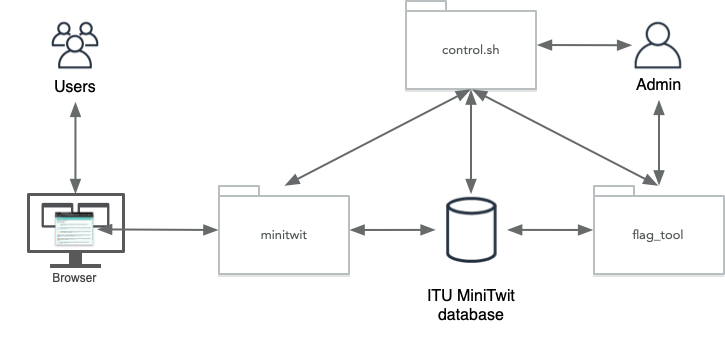
\includegraphics[width=\textwidth]{images/ITU-minitwit-architecture.png}
    \caption{High-level ITU-MiniTwit architexture}
\end{figure}
Detailed Architecture:

\begin{itemize}

\item API Service:

    \subitem Function: Handles all client-server interactions, processing client requests and sending responses back to clients.
    \subitem Implementation: Implemented using Go, indicated by go.mod files, which is suitable for creating performant and scalable backend services.
    \subitem Files: Located within the api directory, which contains all the routing and logic for handling HTTP requests.
\item Database Service:
    \subitem Function: Manages data storage and retrieval, serving as the persistent storage layer for the application.
    \subitem Implementation: Utilizes SQL, as suggested by the presence of schema.sql and query.sql, indicating the use of relational database management systems.
    \subitem Files: The database directory contains scripts and configurations for database setup and management.
\item Front-end:
    \subitem Function: Provides the user interface through which users interact with the ITU-MiniTwit application.
    \subitem Implementation: While specific front-end files weren't listed, typically, this would involve HTML, CSS, and JavaScript files possibly served by the Python service or another static file server.
    \subitem Files: Likely included in the root directory or within a static or templates directory that contains HTML templates and JavaScript files.
\item Containerization and Orchestration:

    \subitem Utilizes Docker, as evidenced by Dockerfile and docker-compose.yml, to containerize the application components, ensuring that each component runs in an isolated environment with its dependencies.
    \subitem Docker Compose helps in defining and running multi-container Docker applications, where services such as the API and database are orchestrated to work together.
\end{itemize}


\section{Dependencies of the Minitwit system}

On the Development Environment:

Vagrant: Used for provisioning virtual environments, ensuring that all developers work within a consistent development environment irrespective of their local machine configurations.
Makefile: Simplifies project builds, allowing developers to automate complex sequences of tasks with simple commands.
Programming Languages and Frameworks:

Python: Used for scripting and possibly serving web content. The requirements.txt file lists all Python library dependencies.
Go: Utilizes modern language features of Go for efficient back-end services.
External APIs and Services:

Prometheus: Employed for monitoring the application’s performance metrics, helping in proactive management and optimization of the application performance.

\section{Important interactions of subsystems}

\section{Current state of the system}

% A description and illustration of the:
% - Design and architecture of your ITU-MiniTwit systems
% - All dependencies of your ITU-MiniTwit systems on all levels of abstraction and development stages. That is, list and briefly describe all technologies and tools you applied and depend on.
% - Important interactions of subsystems
%    - For example, via an illustrative UML Sequence diagram that shows the flow of information through your system from user request in the browser, over all subsystems, hitting the database, and a response that is returned to the user.
%    1- Similarly, another illustrative sequence diagram that shows how requests from the simulator traverse your system.
% - Describe the current state of your systems, for example using results of static analysis and quality assessments.

Lorem ipsum dolor sit amet, consectetur adipiscing elit. Donec venenatis enim a nulla molestie, ac feugiat justo egestas. Nullam interdum lorem et neque ullamcorper volutpat sed sit amet tortor. Praesent sit amet aliquet risus, et accumsan mi. Sed facilisis condimentum varius. Praesent et nunc cursus, laoreet nisi a, venenatis nisl. Integer diam magna, iaculis at dapibus et, rutrum in leo. Pellentesque feugiat diam felis, quis ornare eros dignissim et. Maecenas sed laoreet nunc. Morbi porttitor massa id dui aliquam, non ultrices dolor malesuada.

Cras et porta ex. Lorem ipsum dolor sit amet, consectetur adipiscing elit. Aliquam erat volutpat. Phasellus eget ipsum sit amet nulla porttitor rhoncus at eget elit. Aenean vulputate, urna sed lacinia luctus, sem nisi iaculis nunc, vitae mattis neque sem in felis. Sed tempor tincidunt dapibus. Morbi porta ex erat, sed ornare mi gravida nec. Phasellus ut nunc venenatis, mollis est vestibulum, laoreet nibh. Mauris in vulputate diam. Nunc ullamcorper vestibulum velit, eget volutpat leo vulputate at. Nam in tortor id dolor elementum lobortis at ut elit. Nulla in interdum mi. Sed aliquam ullamcorper blandit.

\chapter{Process' perspective}
% This perspective should clarify how code or other artifacts come from idea into the running system and everything that happens on the way.
% In particular, the following descriptions should be included:
% - A complete description of stages and tools included in the CI/CD chains, including deployment and release of your systems.
% - How do you monitor your systems and what precisely do you monitor?
% - What do you log in your systems and how do you aggregate logs?
% - Brief results of the security assessment and brief description of how did you harden the security of your system based on the analysis
% - Applied strategy for scaling and upgrades
% In case you have used AI-assistants during your project briefly explain which system(s) you used during the project and reflect how it supported/hindered your process.

\section{CI/CD Chain}
We implemented a GitHub Actions workflow to automate the process of testing, building and deploying the most recent version of Minitwit. It is set to execute on each push to the 'Main' branch of our GitHub repository. The workflow is separated into three main jobs: 'BuildAndTest', 'Deploy', and 'Release' which are executed sequentially, each dependent on the last executing successfully.

\subsection{Triggers}
The workflow is triggered on two specific GitHub events: manual triggers via workflow\_dispatch and on pull requests to the main branch. 

\subsection{Jobs}
\subsubsection{BuildAndTest}
In this step all relevant images are built and pushed to the Docker hub and then run and tested to ensure that the system will work as expected. The key steps are as follows:

\begin{enumerate}
    \item \textbf{Checkout:} 
    \begin{itemize}
        \item Uses \texttt{actions/checkout@v2} to fetch the codebase from the repository.
    \end{itemize}
    
    \item \textbf{Environment Setup:} 
    \begin{itemize}
        \item Dynamically creates a \texttt{.env} file with database configurations sourced from GitHub secrets.
    \end{itemize}
    
    \item \textbf{Docker Operations:}
    \begin{itemize}
        \item Logs into Docker Hub using credentials from GitHub secrets to push built images.
        \item Builds and pushes multiple Docker images, including:
        \begin{itemize}
            \item The application image
            \item API image
            \item A test database image
        \end{itemize}
    \end{itemize}
    
    \item \textbf{Python Setup and Dependency Installation:}
    \begin{itemize}
        \item Configures the Python environment.
        \item Installs necessary dependencies to ensure consistent testing conditions.
    \end{itemize}
    
    \item \textbf{Testing:}
    \begin{itemize}
        \item Executes integration tests by setting up the application and its dependencies in Docker containers.
        \item Conducts API tests and application-specific tests to ensure functionality and reliability.
    \end{itemize}
\end{enumerate}

\subsubsection{Deploy}
The \textbf{Deploy} job is activated on successfully completing the \textbf{BuildAndTest} job. This job manages the deployment of the application to the remote server where the application is hosted. The steps are:

\begin{enumerate}
    \item \textbf{Checkout:} 
    \begin{itemize}
        \item Retrieves the latest codebase from the repository, uses \texttt{actions/checkout@v2} similar to the first job.
    \end{itemize}
    
    \item \textbf{SSH Configuration:} 
    \begin{itemize}
        \item Prepares SSH keys to establish a secure connection to the deployment server.
    \end{itemize}
    
    \item \textbf{Deployment Execution:}
    \begin{itemize}
        \item Updates environmental configurations and transfers necessary files to the server using SSH.
        \item Employs Docker Compose on the server to pull the latest Docker images.
        \item Deploys the images using Docker Stack, which effectively updates the running application on the server.
    \end{itemize}
\end{enumerate}

 \subsubsection{Release}
 After the previous jobs have been successfully completed, this job manages software versioning and public release.

 \begin{enumerate}
    \item \textbf{Version Calculation:}
    \begin{itemize}
        \item Executes a script to determine the new version number for automated version tracking.
    \end{itemize}
    
    \item \textbf{GitHub Release Creation:}
    \begin{itemize}
        \item Uses \texttt{actions/create-release@v1} to create a formal release on GitHub.
        \item Tags the release with the new version number and provides release notes outlining the changes in this version.
    \end{itemize}
\end{enumerate}



\section{Monitoring}
For monitoring 

\section{Logging}

\section{Security assessment}

\section{Scaling strategy}

\chapter{Lessons Learned Perspective}

\section{Evolution and refactoring}

\section{Operation}

\section{Maintenance}

% Describe the biggest issues, how you solved them, and which are major lessons learned with regards to:
% - evolution and refactoring
% - operation, and
% - maintenance
% of your ITU-MiniTwit systems. Link back to respective commit messages, issues, tickets, etc. to illustrate these.
% Also reflect and describe what was the "DevOps" style of your work. For example, what did you do differently to previous development projects and how did it work?

Lorem ipsum dolor sit amet, consectetur adipiscing elit. Donec venenatis enim a nulla molestie, ac feugiat justo egestas. Nullam interdum lorem et neque ullamcorper volutpat sed sit amet tortor. Praesent sit amet aliquet risus, et accumsan mi. Sed facilisis condimentum varius. Praesent et nunc cursus, laoreet nisi a, venenatis nisl. Integer diam magna, iaculis at dapibus et, rutrum in leo. Pellentesque feugiat diam felis, quis ornare eros dignissim et. Maecenas sed laoreet nunc. Morbi porttitor massa id dui aliquam, non ultrices dolor malesuada.

Cras et porta ex. Lorem ipsum dolor sit amet, consectetur adipiscing elit. Aliquam erat volutpat. Phasellus eget ipsum sit amet nulla porttitor rhoncus at eget elit. Aenean vulputate, urna sed lacinia luctus, sem nisi iaculis nunc, vitae mattis neque sem in felis. Sed tempor tincidunt dapibus. Morbi porta ex erat, sed ornare mi gravida nec. Phasellus ut nunc venenatis, mollis est vestibulum, laoreet nibh. Mauris in vulputate diam. Nunc ullamcorper vestibulum velit, eget volutpat leo vulputate at. Nam in tortor id dolor elementum lobortis at ut elit. Nulla in interdum mi. Sed aliquam ullamcorper blandit.
\end{spacing}

\end{document}
